\documentclass[border=2pt,tikz]{standalone}
% \documentclass{article}

% \usepackage[vmargin=10mm]{geometry}
% \usepackage{tikz}
\usetikzlibrary{arrows,automata,positioning}
\tikzset{
    every picture/.style={
        semithick,shorten >=1pt,>=stealth',node distance=4em,
        every state/.style={minimum size=1em,align=center},
        accepting/.style={double distance=.1em,outer sep=\pgflinewidth}
    }
}
\usepackage[fontset=ubuntu]{ctex}
\begin{document}

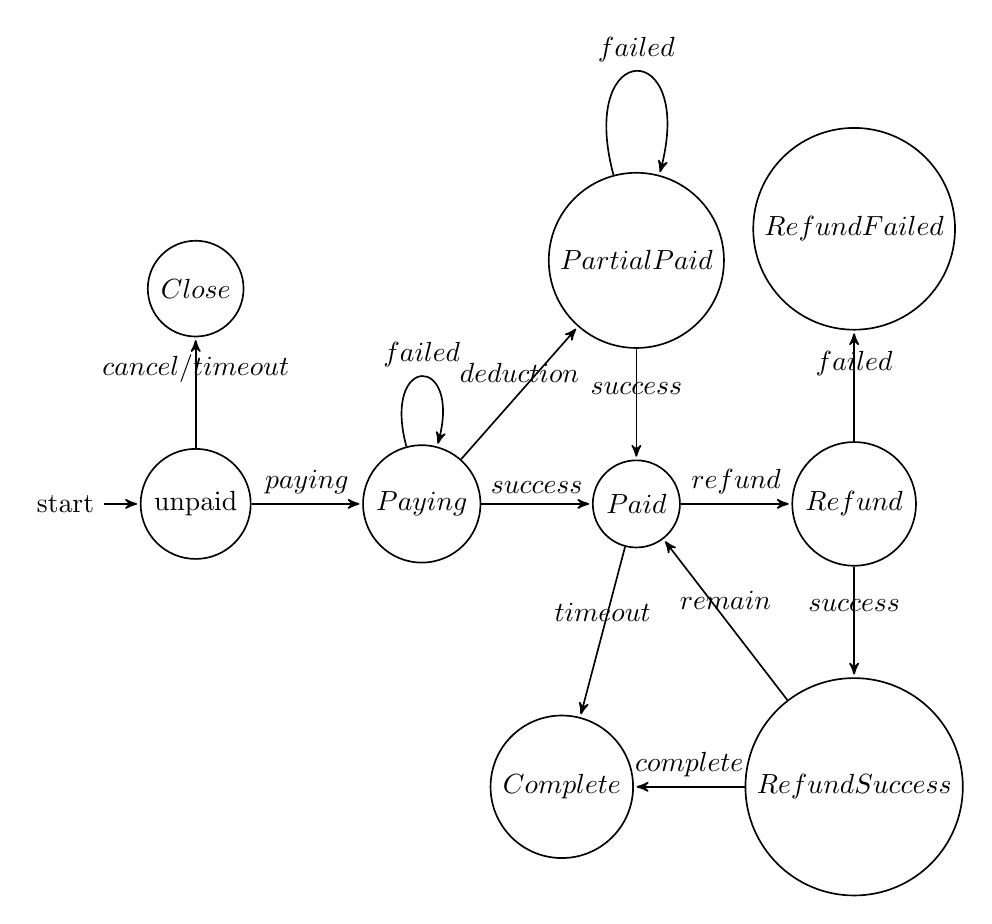
\begin{tikzpicture}
    \node[state,initial]   (0) {unpaid};
    \node[state]           (1) [above=of 0] {$Close$};
    \node[state]           (3) [right=of 0] {$Paying$};
    \node[state]           (5) [right=of 3] {$Paid$};
    \node[state]           (10) [above=of 5] {$Partial Paid$};
    \node[state]           (6) [right=of 5] {$Refund$};
    \node[state]           (7) [above=of 6] {$Refund Failed$};
    \node[state]           (9) [below=of 6] {$Refund Success$};
    \node[state]           (8) [left=of 9] {$Complete$};
    \path[->](0) edge [above] node         {$cancel/timeout$}    (1)
             (0) edge [above] node         {$paying$}    (3)
             (3) edge [loop above] node         {$failed$}    (3)
             (3) edge [above] node         {$success$}   (5)
             (5) edge [above] node         {$refund$}    (6)
             (6) edge [above] node         {$failed$}    (7)
             (6) edge [above] node         {$success$}  (9)
             (9) edge [above] node         {$complete$}  (8)
             (9) edge [above] node         {$remain$}  (5)
             (5) edge [above] node         {$timeout$}  (8)
             (3) edge [above] node         {$deduction$}  (10)
            (10) edge [above] node         {$success$}  (5)
             (10) edge [loop above] node         {$failed$}    (10)
              ;
\end{tikzpicture}

\end{document}
